\section{Triangulated Manifolds}

\begin{definition}
    We define the \textbf{standard closed $k$-simplex} in $\R^{k+1}$ to be the
    set $[e_0, \dots, e_k]$ of all affine combinations of the standard
    basis $\{e_0, \dots, e_k\}$ of $R^{k+1}$. That is,
    \begin{equation*}
        [e_0, \dots, e_k]=\{a_0e_0+\dots+a_ke_k : a_i \geq 0 \text{ for all }
        0 \leq i \leq k \text{ and } \sum_{i=0}^k{a_i}=0\}
    \end{equation*}
    When the basis is understood, we simply write $[s]$. We define the
    \textbf{standard open $k$-simplex} in $\R^{k+1}$, $(e_0, \dots, e_k)$ to be
    the interior of $[e_0, \dots, e_k]$; that is
     \begin{equation*}
        (e_0, \dots, e_k)=\{a_0e_0+\dots+a_ke_k : a_i>0 \text{ for all }
        0 \leq i \leq k \text{ and } \sum_{i=0}^k{a_i}=0\}
    \end{equation*}
    again, when the basis is clear, we write $(s)$. We denote the
    \textbf{dimension} of $[e_0, \dots, e_k]$ and $(e_0, \dots, e_k)$ to be
    \begin{equation*}
        \dim{[e_0, \dots, e_k]}=\dim{(e_0, \dots, e_k)}=k
    \end{equation*}
\end{definition}

\begin{example}\label{example_1.11}
    The standard $0$-simplex is the point set  $\{1\}$ of $\R$.
\end{example}

\begin{definition}
    We define a \textbf{$k$-simplex} in a topological space $X$ to be a
    continuous map  $f:[s] \xrightarrow{} X$ such that $[s]$ is the standard
    $k$-simplex, and  $f|_{(s)}$ is homeomorphic onto its image $f|_{(s)}((s))$.
    We define an \textbf{open $k$-simplex} to be the restriction of a
    $k$-simplex from  $[s]$ to its interior $(s)$. We denote the
    \textbf{dimension} of a $k$-simplex  $f$ to be
    \begin{equation*}
        \dim{f}=\dim{[s]}
    \end{equation*}
\end{definition}

\begin{example}\label{example_1.12}
    \begin{enumerate}
        \item[(1)] The standard $1$-simplex, shown in figure \ref{figure_1.7}
            consists of a line segment in $\R^2$ with vertices $(1,0)$ and $(0,1)$.
            It can be shown to be homeomorphic to an interval. Figure
            \ref{figure_1.8} also shows a $1$-simplex  $f:[e_0,e_1]
            \xrightarrow{} X$.
            \begin{figure}[h]
                \centering
                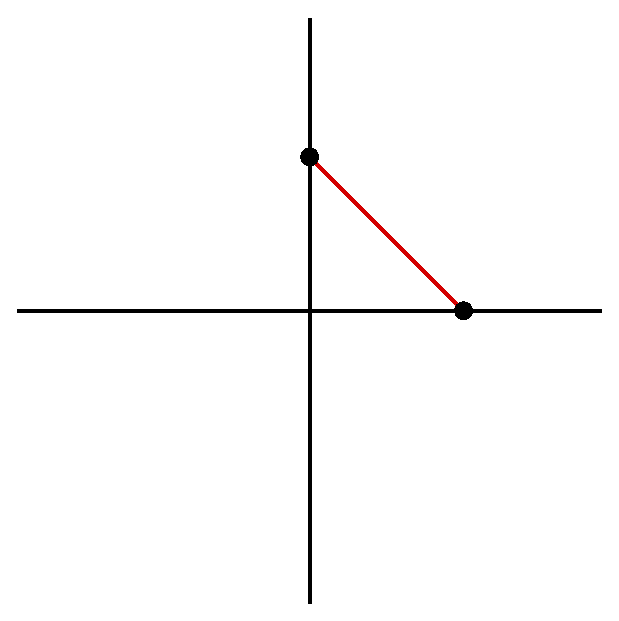
\includegraphics[scale=0.5]{Figures/Chapter1/standard_1_simplex.eps}
                \caption{The standard $1$-simplex  $[e_0,e_1]$.}
                \label{figure_1.7}
            \end{figure}

        \item[(2)] The standarde $2$ simplex is a triangle in  $\R^3$ with
            vertices  $(1,0,0)$, $(0,1,0)$, and $(0,0,1)$.
            \begin{figure}[h]
                \centering
                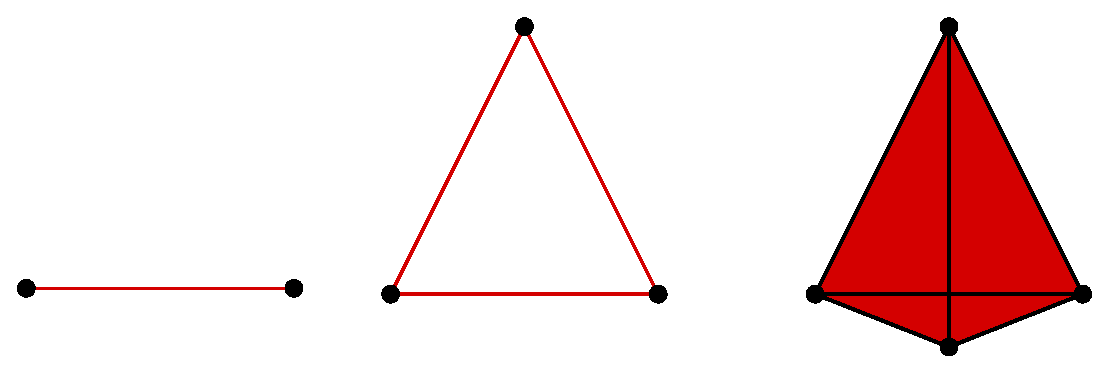
\includegraphics[scale=0.5]{Figures/Chapter1/simplices.eps}
                \caption{A $1$-simplex, a  $2$-simplex, and a  $3$-simplex}
                \label{figure_1.8}
            \end{figure}
            It can be visualized in figure \ref{figure_1.8} to be a $2$-simplex,
            which is just a map  $f:[e_0,e_1,e_2] \xrightarrow{} X$.

        \item[(3)] The standard $3$-simplex is a tetrahedron  (in $\R^4$) with
            vertices at $(1,0,0,0)$, $(0,1,0,0)$, $(0,0,1,0)$, and $(0,0,0,1)$.
            Figure \ref{figure_1.8} again shows a $3$-simplex.
    \end{enumerate}
\end{example}

\begin{definition}
    For $0 \leq i \leq j$, we define a \textbf{$j$-face} of a $k$-simplex
     $f:[s] \xrightarrow{} X$ to be a subset of the form
     \begin{equation*}
         \{a_0e_0+\dots+a_ke_k : a_{i_1}=\dots=a_{i_j}=0\}
     \end{equation*}
     We denote the \textbf{dimension} of a face to be  $k-j$. We call a
     $0$-face a  \textbf{vertex}, and a $1$-face an  \textbf{edge}.
\end{definition}

\begin{lemma}\label{1.4.1}
    Let $f:[s] \xrightarrow{} X$ be a $k$ simplex, for any topological space
    $X$. Then a  $j$ face of $f$ is a $k-j$ simplex.
\end{lemma}

\begin{example}\label{example_1.13}
    \begin{enumerate}
        \item[(1)] $0$-simpleces have only themselves as faces.

        \item[(2)] The standard $1$-simplex  $[e_0,e_1]$ has only the set
            $\{e_0,e_1\}$ as a $1$-face, and has the point sets  $\{e_0\}$
            and $\{e_1\}$ as its $0$-faces.

        \item[(3)] A $2$-simplex has one  $2$-face, three $1$-faces, and three
            $0$-faces. A $3$-simplex has one $3$-face, four $2$-faces, six
            $1$-faces, and four $0$-faces.
    \end{enumerate}
\end{example}

\begin{definition}
    A \textbf{simplicial complex} based on a topologica space $X$ is a set  $K$
    of simplices  $f:[s] \xrightarrow{} X$ such that
    \begin{enumerate}
        \item[(1)] For any simplex $f \in K$, the faces of $f$ are in  $K$.

        \item[(2)] For any pair of simplices $f_1, f_2 \in K$, if the
            intersection of the images of $f|_{(s_1)}$ and $f_2|_{(s_2)}$ is
            nonempty, then the images are the same.
    \end{enumerate}
    We define the \textbf{dimension} of $K$ to be  $\dim{K}=\sup\{\dim{f_i}\}$,
    for all $f_i \in K$, and we call the union of the images of simplices in
    $K$ the  \textbf{underlying space}, and denote it $\|K\|$.
\end{definition}

\begin{figure}[h]
    \centering
    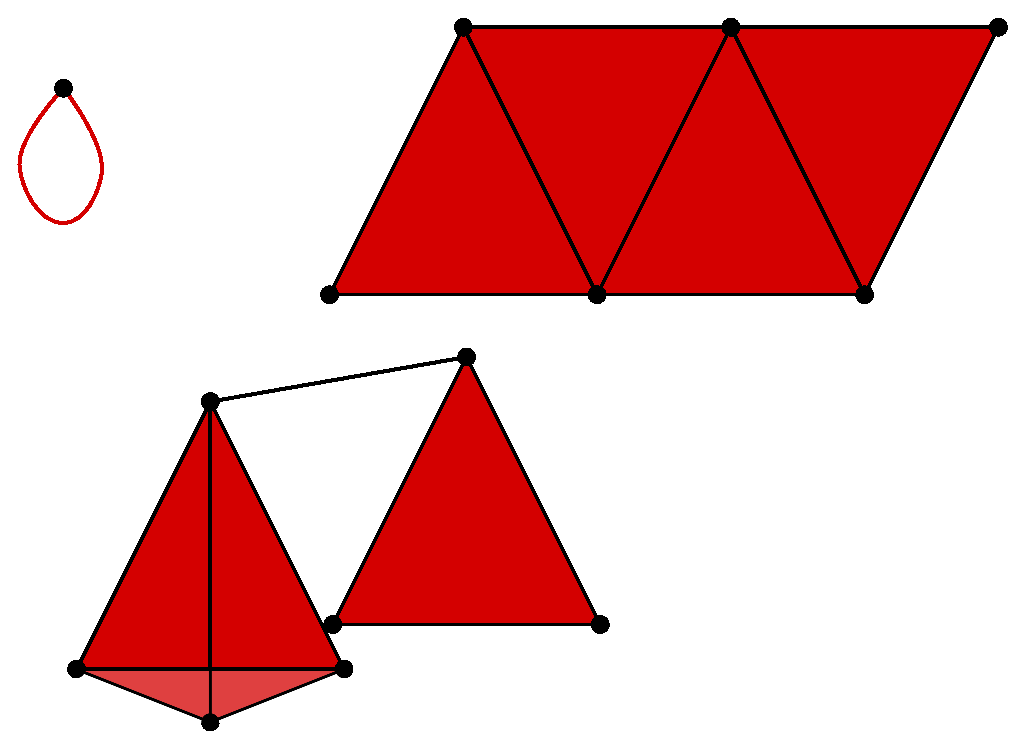
\includegraphics[scale=0.5]{Figures/Chapter1/simplicial_complexes.eps}
    \caption{A collection of simplicial complexes.}
    \label{figure_1.9}
\end{figure}

\begin{definition}
    A \textbf{triangulated $n$-manifold} is a topological $n$-manifold $M$,
    together with a simplicial comlex  $K$ based in  $M$ such that
    \begin{enumerate}
        \item[(1)] The underlying space of $K$ is  $M$; i.e.  $\|K\|=M$.

        \item[(2)] $K$ is locally finite; i.e. if  $C$ is a compact subset of
            $M$, then the set of all nonempty intersections  $C \cap f([s])$ is
            finite, where $f \in K$.

        \item[(3)] For complexes $f,g \in K$, restricted to open simplices, the
            composition  $\inv{g} \circ f$ is affine on its domain.
    \end{enumerate}
    We call $K$ a  \textbf{triangulation} of $M$, and for any simplex $f:[s]
    \xrightarrow{} M$, we call the pair $(f([s]),\inv{f})$ a \textbf{simplicial
    chart} of $K$. Writing $K=\{f_\a\}$, we also call  $f_\a$ a
    \textbf{simplex} of $M$, for each  $\a$.
\end{definition}

\begin{example}\label{example_1.14}
    \begin{enumerate}
        \item[(1)] We have the triangulation of the sphere $S^2$ and the torus
            $T^2$ as show in figure \ref{figure_1.9}.
            \begin{figure}[h]
                \centering
                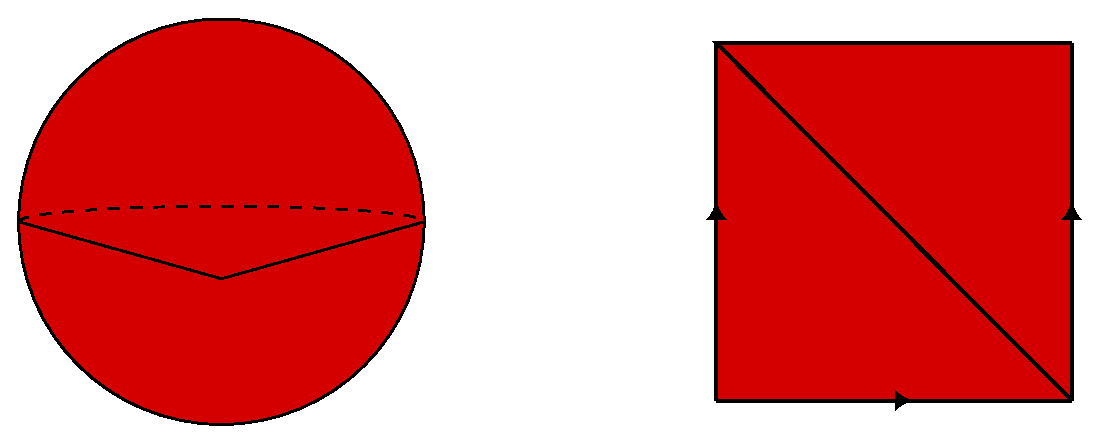
\includegraphics[scale=0.5]{Figures/Chapter1/trangulations_S^2_T^2.eps}
                \caption{}
                \label{figure_1.10}
            \end{figure}

        \item[(2)] The following figure \ref{figure_1.11} shows a triangulated
            cube. This is a portion of the triangulation of the $3$-torus
            $T^3$. The triangulation of  $T^3$ is taken by indentifying  $8$
            appropriately selected reflections of the given cube. The resulting
            triangulation has forty $3$-simplices.
            \begin{figure}[h]
                \centering
                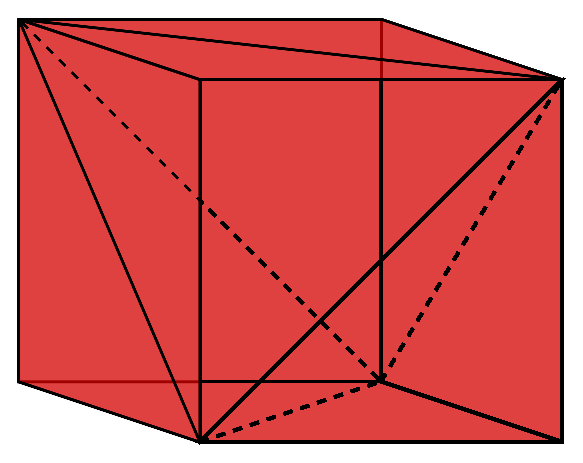
\includegraphics[scale=0.5]{Figures/Chapter1/trangulation_T^3.eps}
                \caption{}
                \label{figure_1.11}
            \end{figure}
    \end{enumerate}
\end{example}

\begin{theorem}\label{1.4.2}
    Every compact $1$-manifold admits a triangulation.
\end{theorem}

\begin{theorem}[Rad\'o \& Kerekjarto]\label{1.4.3}
    Every compact $2$-manifold admits a triangulation.
\end{theorem}

\begin{theorem}[Bing \& Moise]\label{1.4.4}
    Every compact $3$-manifold admits a triangulation.
\end{theorem}

\begin{definition}
    Let $K$ and  $L$ be simplicial complexes. We call a continuous map
    $\phi:\|K\| \xrightarrow{} \|L\|$ a \textbf{simplicial map} if for every
    simplex $f$ in $K$, there exists  a simplex $g$ in  $L$, such that  $\phi
    \circ f=g$.
\end{definition}

\begin{figure}[h]
    \centering
    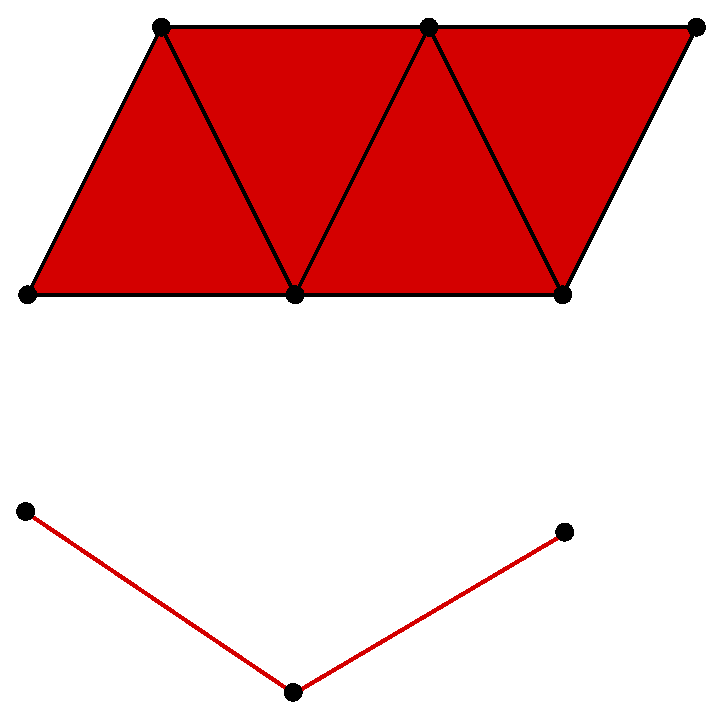
\includegraphics[scale=0.5]{Figures/Chapter1/simplicial_map.eps}
    \caption{A simplicial map between a simplicial complex of $2$-simplices, and
    a simplicial complex of  $1$-simplices.}
    \label{figure_1.12}
\end{figure}

\begin{definition}
    Let $K$ and  $L$ be simplicial complexes, and  $\phi:\|K\| \xrightarrow{}
    \|L\|$ a simplicial map. We call $\phi$ a simplicial isomorphism if it is a
    homeomorphism and we call  $K$ and  $L$  \textbf{isomorphic} if there exists
    a simplicial isomorphism between them,
\end{definition}

\begin{definition}
    Let $(M,K)$ and $(N,L)$ triangulated manifolds. We call them
    \textbf{isomorphic} if there exists a simplicial isomorphism $\phi:M
    \xrightarrow{} N$.
\end{definition}

\begin{definition}
    We define a \textbf{subcomplex} of a simplicial complex $K$ to be a subset
    $L$ of  $K$ that is also a simplicial complex.
\end{definition}

\begin{definition}
    Let $K$ be a finite simplicial complex and $S_i$ the collection if simplices
    of dimension $i$. We define the \textbf{Euler characteristic} of $K$ to be
    \begin{equation*}
        \chi(K)=\sum_{i=0}^n{(-1)|S_i|}
    \end{equation*}
\end{definition}
